\Chapter{Deep Convolutional GAN példa}

Ezen architektúra természetesen a mai eredmények mellett egyszerűnek tűnhet elsőre, viszont a későbbi, fejlettebb architektúrákban többségében megfigyelhető, hogy erre építkeztek. Természetesen az architektúra egy igen egyszerű kiegészítést kínált az eredeti GAN hálózatra: konvolúciós rétegeket alkalmaz a rejtett rétegekben mind a Generátor, mind a Diszkriminátor esetében. A konvolúciós rétegek segítségével a képeken lévő összefüggő pixelek kapcsolatairól pontosabb reprezentációt kaphatunk, így képek generálásához is hasznos lehet a módszer.

\begin{figure}[h]
\centering
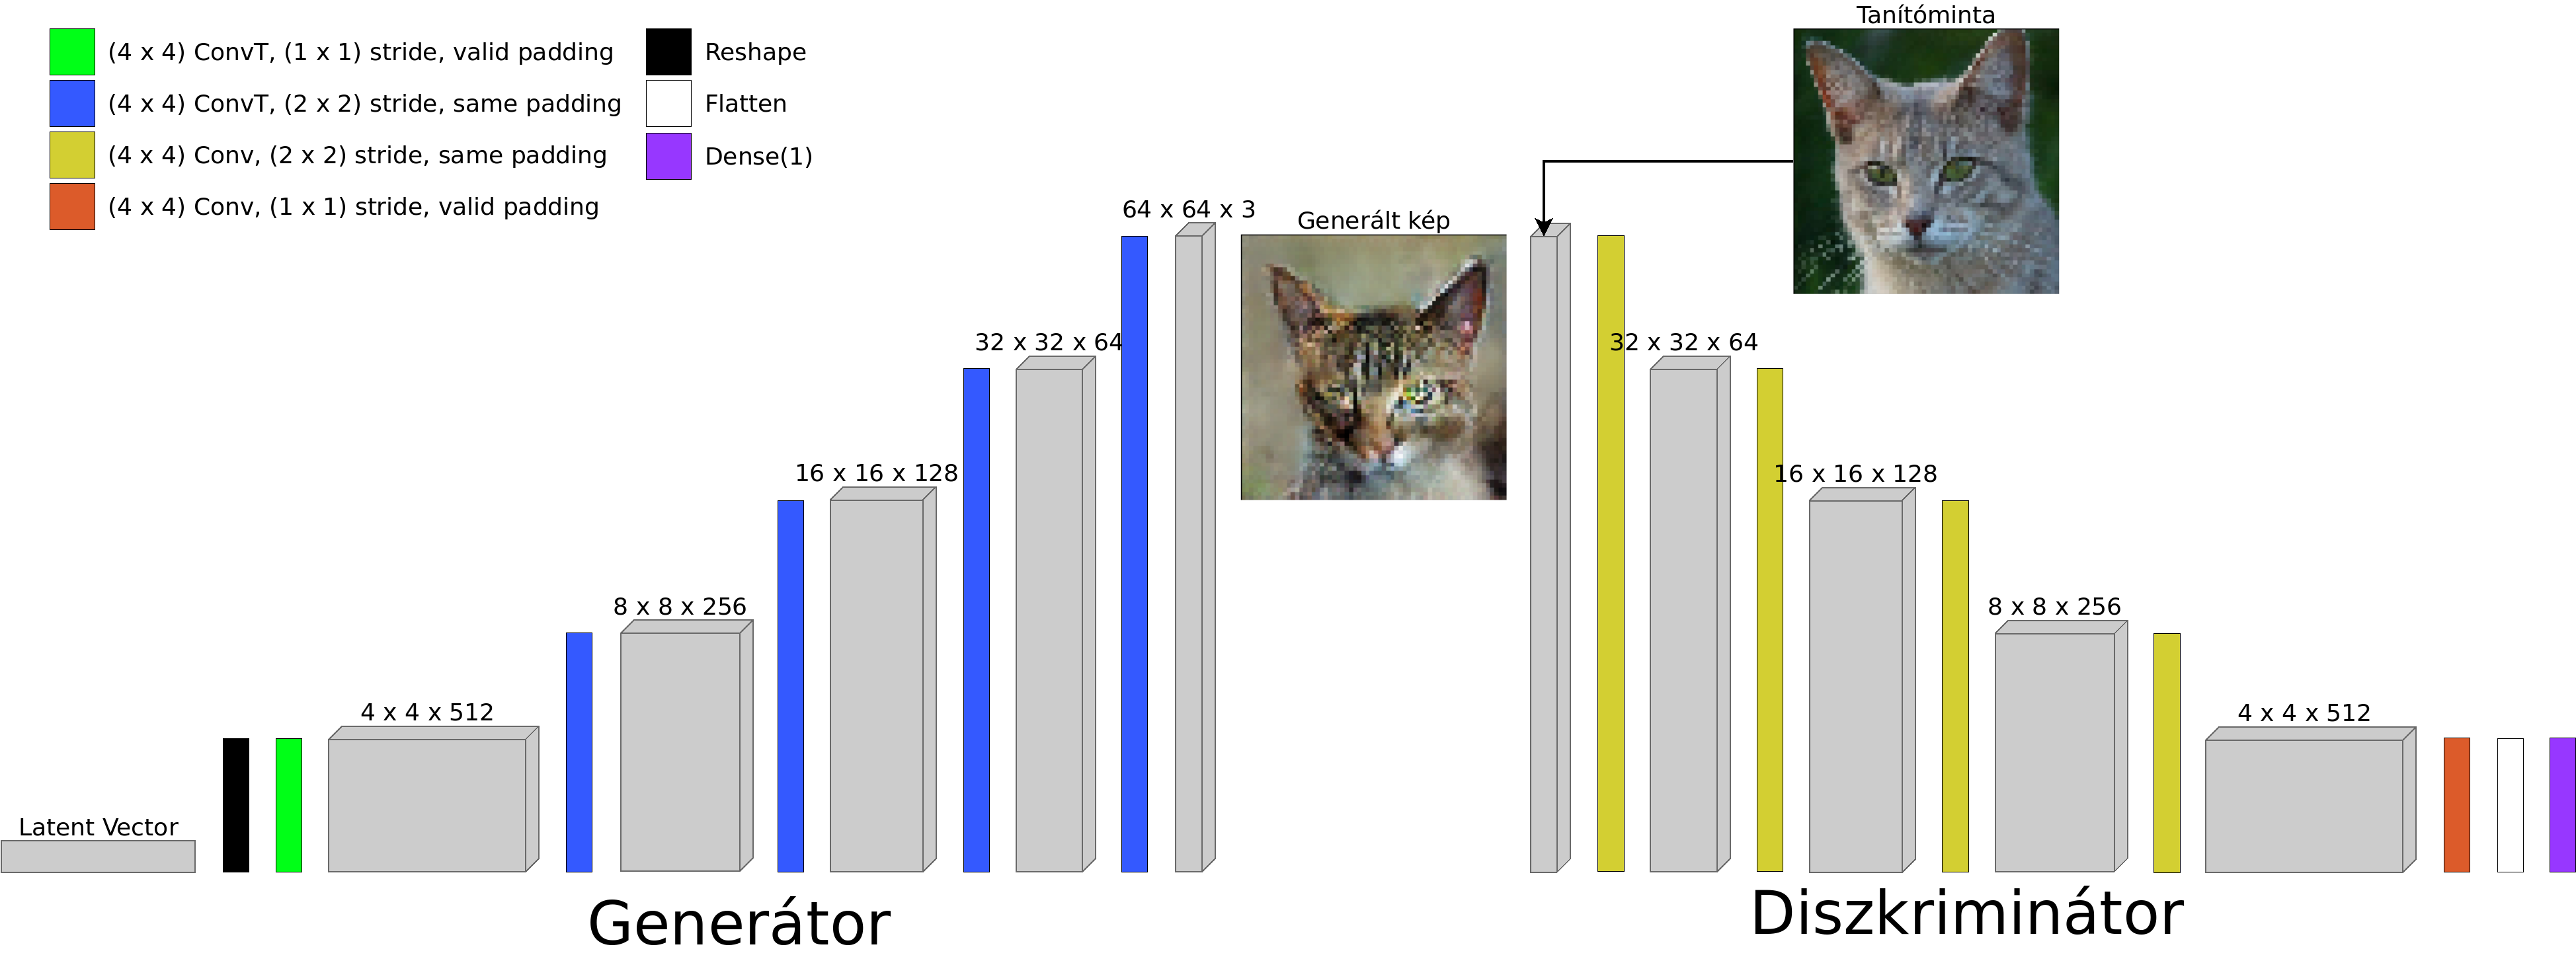
\includegraphics[width=15cm]{images/DCGAN.png}
\caption{DCGAN architektúra}
\label{fig:dcgan}
\end{figure}

\Section{Generátor}

Az osztályozáshoz használt konvolúciós hálókkal ellentétben a Generátorban a kisebb felbontás felől haladunk a nagyobb felbontásig.
A generátor modellem első implementációjában Dekonvolúciós rétegeket alkalmaztam, amelyet Transzponált konvolúciós rétegnek is nevezhetünk. A Dekonvolúciós rétegek segítségével minden rejtett réteg kimenete egy nagyobb felbontású kép lesz, ellentétben a konvolúció működésével. Tehát a hálónak jelen esetben meg kell tanulnia a rétegekben az optimális felbontás-növelést. Előre megadott paraméterek a filterek darabszáma, a kernel mérete, a strides(?) és a padding. Ha a padding-ot "same"-re és ha a strides paramétert 2x2-esnek választjuk, úgy a réteg kimenetén megjelenő kép felbontása kétszerese lesz a bemeneti oldalon megfigyelhető képnek. A rejtett rétegekben kezdetben ReLU aktivációs függvényt használtam, a neuronok kezdő értékeit a He inicializációs technikával állítottam be (Hands on könyv ajánlása alapján).

\begin{figure}[h]
\centering
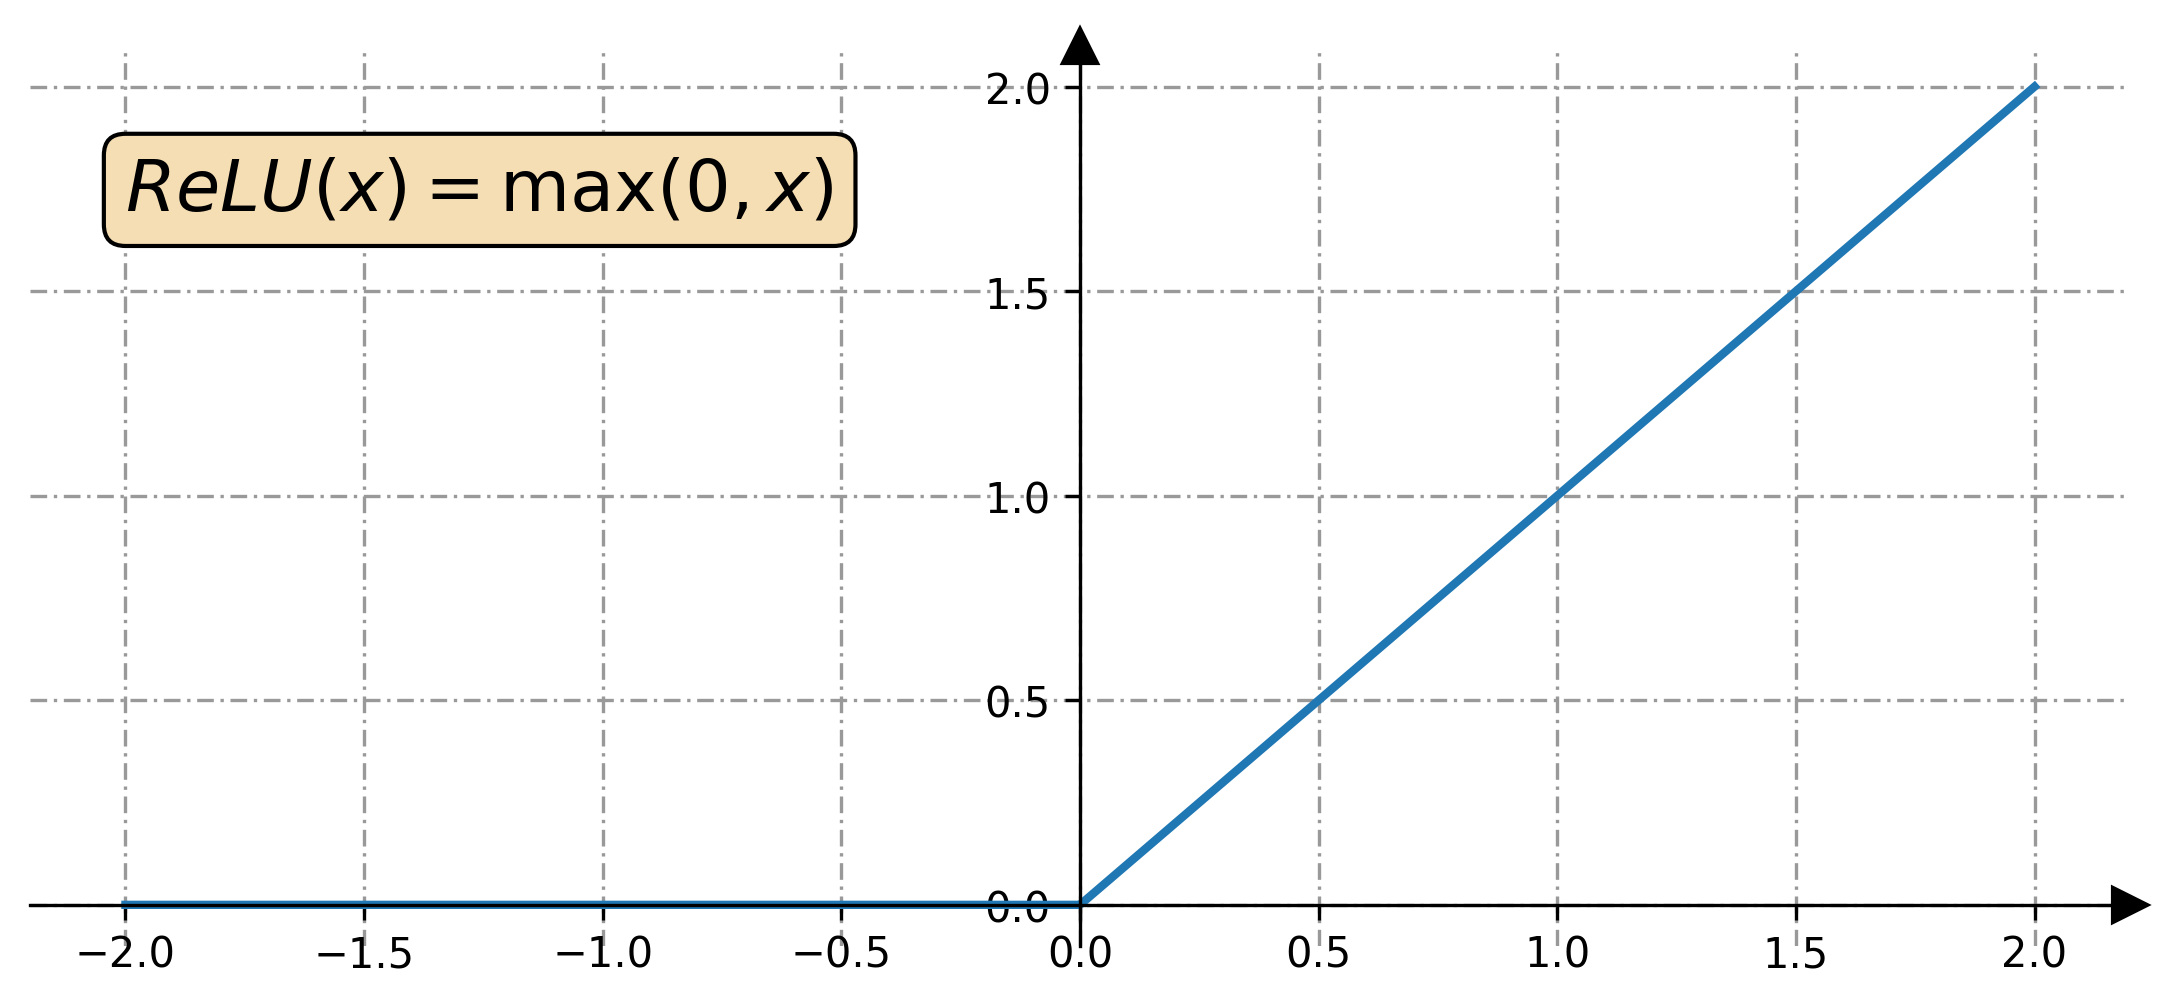
\includegraphics[width=10cm]{images/relu.png}
\caption{ReLU aktivációs függvény}
\label{fig:relu}
\end{figure}

A tanításhoz célszerű a kép pixeleinek intenzitását normalizálni a [-1, 1] intervallumra. A Generátor is ebben az intervallumban fogja a képek pixeleit generálni a hiperbolikus tanges kimeneti aktivációs függvényéből adódóan. (tanh indoklás, sigmoid helyett..) A megjelenítéshez később természetesen denormalizálnunk kell a generált képek pixelértékeit a [0, 255] tartományra.

A Generátor modell bemenetként az előre definiált látens tér dimenziójával megegyező dimenziójú zajt kap. Majd ezen bemeneti zaj segítségével állítja össze a megfelelő kimeneti képet. A tanulás során tehát a látens tér tartományaihoz rendeli a tanult jellegzetességeket és a látens teret mintavételezve dekódolható a Generátor segítségével a ponthoz tartozó kép.

A bemeneti zaj egy Reshape rétegen megy keresztül, amelyben a látens tér dimenziószámát átformázza egy 1x1xLdim dimenziójú mátrixá. Ezen réteg kimenetével a későbbi dekonvolúciós rétegek már tudnak dolgozni.
Ezután az első dekonvolúciós rétegen megy át a kapott mátrix, amely 512 darab filtert tartalmaz, 4x4-es kernelméretekkle dolgozik és 'valid' paddingot használ. Az aktivációs függvénye ReLU a már említett He inicializálással. Ezen lépés arra szolgál, hogy a látens térből előállítson egy 4x4x512-es tensort, amely az első, legkisebb felbontású képünknek tekinthetjük ebben az esetben, ahol a színcsatornák száma 512 és a felbontása 4x4.

A Generátorban ezután 2x2-es stride értékeket használva a kívánt felbontásig dekonvolúciós rétegeken keresztül növekszik a felbontás. A kernel méretét a rétegekben egységesen 4x4-ra állítottam be, a paddig 'same' és a strides a már említett 2x2-es. Az aktivációs függvény szintén ReLU. A rétegekben haladva a filterek darabszáma pedig feleződik. A filterek optimális számára csupán csak empirikus eredményeket találtam. Az utolsó dekonvolúciós réteg 3 darab filterrel rendelkezik.

A kimeneti képnek olyan tulajdonságokkal kell rendelkeznie, mint a tanítómintában szeplő képeknek. Például ha a tanítóminta színes képekből áll, rgb színkeveréssel, vagyis három színcsatornával, úgy a Generátor kimenetén is ilyen képekre van szükségünk. Mivel az említett dekonvolúciós rétegek több mint 3 színcsatornával dolgoztak, a megjeleníthetőség miatt szükséges tehát az utolsó dekonvolúciós rétegben a 3 darab filter.
Végül a hiperbolikus tangens aktivációs függvény hatására az eredményeket a [-1, 1] intervallumba transzformálja.

\begin{figure}[h]
\centering
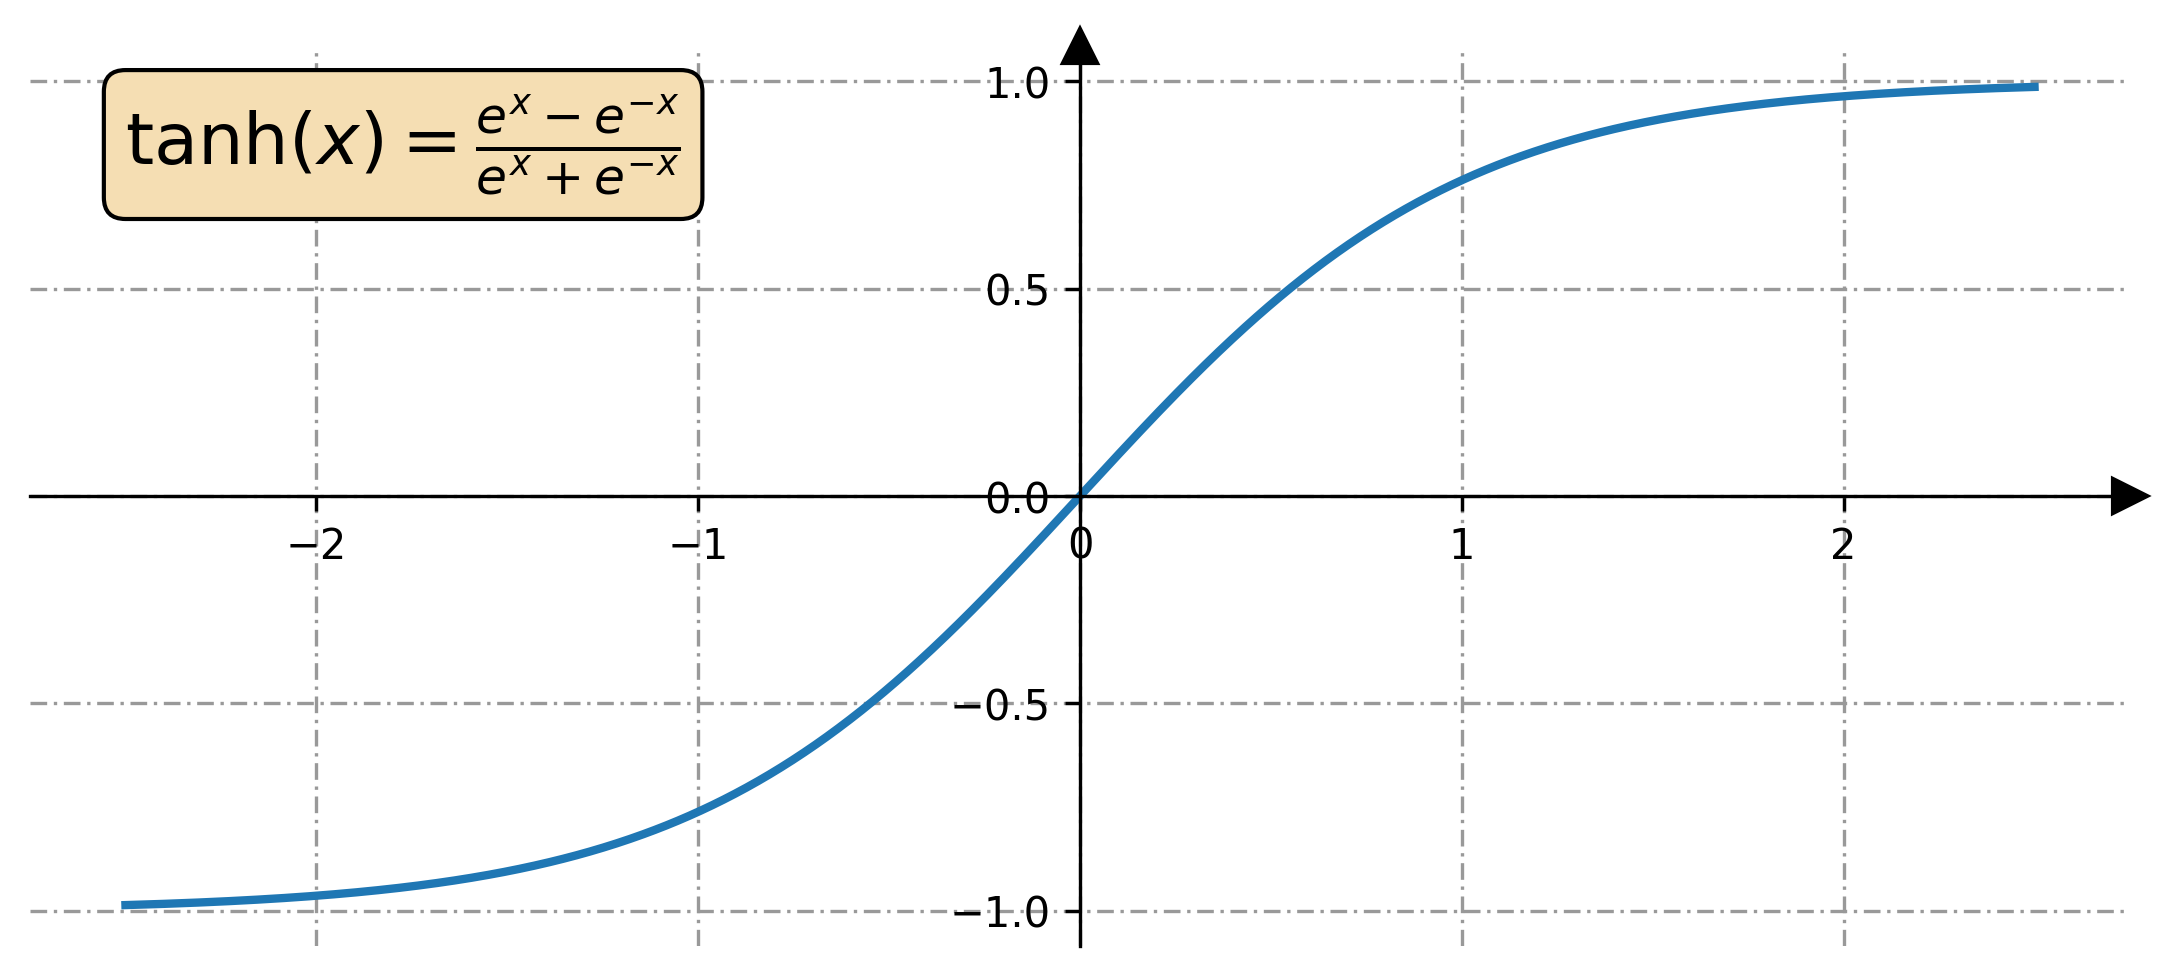
\includegraphics[width=10cm]{images/tanh.png}
\caption{Hiperbolikus tangens aktivációs függvény}
\label{fig:tanh}
\end{figure}

\begin{python}
def add_upsampling_unit(model,
                        filters, kernel_size, strides, padding):
    model.add(
        Conv2DTranspose(
            filters=filters, kernel_size=kernel_size,
            strides=strides,
            padding=padding, activation="relu",
            kernel_initializer="he_normal"
        )
    )
    
def make_generator_model(latent_dim):
    model = Sequential()
    model.add(Reshape((1, 1, 100), input_shape=[latent_dim]))
    add_upsampling_unit(model, 512, 4, (1, 1), 'valid')
    add_upsampling_unit(model, 256, 4, (2, 2), 'same')
    add_upsampling_unit(model, 128, 4, (2, 2), 'same')
    add_upsampling_unit(model, 64, 4, (2, 2), 'same')
    model.add(Conv2DTranspose(filters=3, kernel_size=4,
                              strides=(2, 2), padding='same'))
    model.add(Activation("tanh"))
    return model
\end{python}

\Section{Diszkriminátor}

A Diszkriminátor modell lényegében egy bináris osztályozó, amely eldönti, hogy a bemenetül kapott kép valódi vagy hamis. A bemeneti kép konvolúciós rétegeken megy végig, majd a kimeneti rétegen sigmoid aktivációs függvény segítségével hozza meg a döntést. A konvolúciós rétegek segítségével a modell fel tudja tárni a képeken található jellegzetességeket. A képen található mintázatokat filterek segítségével tanulja meg, amelyek megadott kernelméretekben pásztázzák végig a bemenetet. Így az egyes konvolúciósrétegek kimeneteként egy olyan reprezentáció jön létre a bemeneti képről, amelyben érvényesülnek a pixeleket körülölelő további pixelek kapcsolatai is. Ezáltal a kimeneti aktivációs függvény előtti réteg, a szerializáció (Flattening) kevésbé fogja a kép tartalmára vonatkozó információt rontani. Mivel a tanítóminta képeinek pixelértékeit normalizáltuk a [-1, 1] intervallumra, így a diszkriminátor a bemenetén is ilyen tulajdonságú képeket vár. A Diszkriminátor felépítésben hasonlít a Generátorhoz, lényegében annak tükörképeként képzelhetjük el. Viszont a dekonvolúciós rétegek helyett konvolúciós rétegeket alkalmazunk benne.

\begin{python}
def add_downsampling_unit(model, filters,
                          kernel_size, strides, padding):
    model.add(
        Conv2D(
            filters=filters, kernel_size=kernel_size,
            strides=strides, padding=padding, activation="relu",
            kernel_initializer="he_normal"
        )
    )

def make_discriminator_model():
    model = Sequential()
    model.add(
        Conv2D(
            filters=64, kernel_size=4, strides=2,
            input_shape=(64, 64, 3),
            padding="same", activation="relu",
            kernel_initializer="he_normal"
        )
    )
    add_downsampling_unit(model, filters=128,
                          kernel_size=4, strides=2, padding="same")
    add_downsampling_unit(model, filters=256,
                          kernel_size=4, strides=2, padding="same")
    add_downsampling_unit(model, filters=512,
                          kernel_size=4, strides=2, padding="same")
    model.add(
        Conv2D(
            filters=100, kernel_size=4, strides=1, padding="valid",
            activation="relu"
        )
    )
    model.add(Flatten())
    model.add(Dense(1))
    return model
\end{python}

\begin{tabular}{ |p{6cm}||p{4cm}|p{3cm}|  }
	\hline
	\multicolumn{3}{|c|}{\textbf{Generátor}} \\
	\hline
	Réteg & Aktivációs függvény & Kiement alakja\\
	\hline
	Input & - & (100)\\
	Reshape & - & (1, 1, 100)\\
	(4x4) ConvT, (1x1) stride, valid & ReLU & (4, 4, 512)\\
	(4x4) ConvT, (2x2) stride, same & ReLU & (8, 8, 256)\\
	(4x4) ConvT, (2x2) stride, same & ReLU & (16, 16, 128)\\
	(4x4) ConvT, (2x2) stride, same & ReLU & (32, 32, 64)\\
	(4x4) ConvT, (2x2) stride, same & tanh & (64, 64, 3)\\
	\hline
	\multicolumn{3}{|r|}{Paraméterek száma: \textbf{3.5 millió}} \\
	\hline
\end{tabular}


\begin{tabular}{ |p{6cm}||p{4cm}|p{3cm}|  }
	\hline
	\multicolumn{3}{|c|}{\textbf{Diszkriminátor}} \\
	\hline
	Réteg & Aktivációs függvény & Kiement alakja\\
	\hline
	Input & - & (64, 64, 3)\\
	(4x4) Conv, (2x2) stride, same & ReLU & (32, 32, 64)\\
	(4x4) Conv, (2x2) stride, same & ReLU & (16, 16, 128)\\
	(4x4) Conv, (2x2) stride, same & ReLU & (8, 8, 256)\\
	(4x4) Conv, (2x2) stride, same & ReLU & (4, 4, 512)\\
	(4x4) Conv, (1x1) stride, valid & ReLU & (1, 1, 100)\\
	Flatten & - & (100)\\
	Dense(1) & - & (1)\\
	\hline
	\multicolumn{3}{|r|}{Paraméterek száma: \textbf{3.5 millió}} \\
	\hline
\end{tabular}

\Section{Tanítás, mérések}
A felvázolt architektúrát tanítva a hibaértékek a következő ábrához hasonlóan alakulnak:

\begin{figure}[h]
\centering
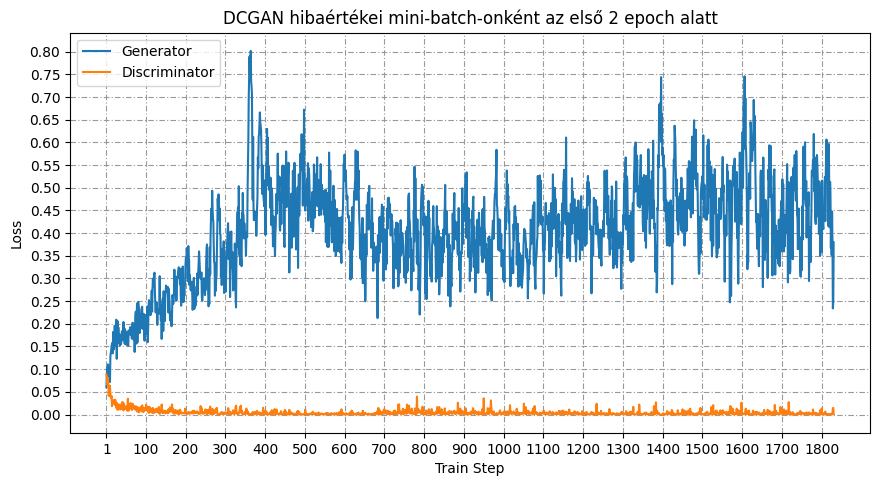
\includegraphics[width=15cm]{images/miniloss.png}
\caption{Hibaértékek mini-batch-onként}
\label{fig:mini-batch_loss_plot}
\end{figure}

A modell tanítása nehézkes lehet, ezt kívánom szemléltetni a fenti ábrákkal.
Jól látható, hogy a tanítási folyamat során igen érdekes hibaértékek születnek. Egy tanítási lépés egy minibatch-on történő tanítást jelent, egy epoch pedig az összes minibatch-on való tanítást jelenti.
Ha csak a nyers hibaértékre tekintünk, akkor azt figyelhetjük meg, hogy a tanítási lépések között erősen oszcillálnak az értékek. Kijelenthetjük a látott eredmények alapján, hogy a tanítás valóban nem stabil és egészen random módon változhatnak az értékek.
A szemléltetés kedvéért a következő ábrán a minibatchokon számolt hibaértékek átlagait figyelhetjük meg epoch-onként.

\begin{figure}[h]
\centering
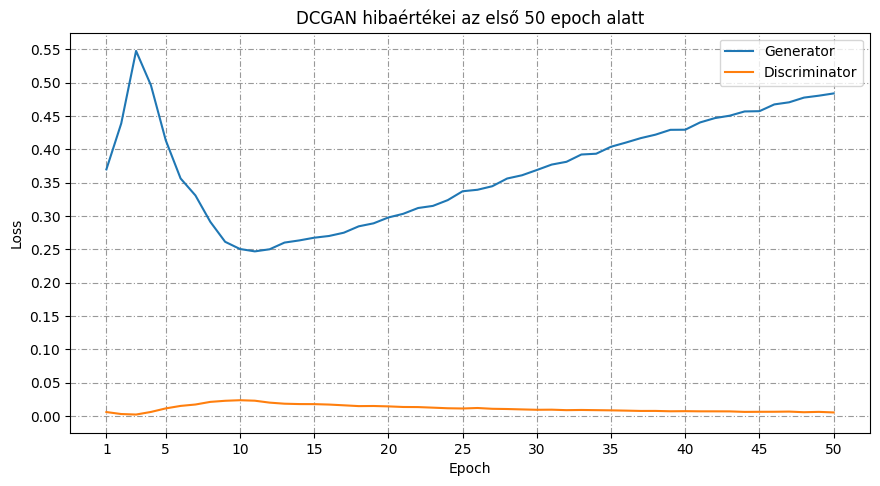
\includegraphics[width=15cm]{images/epochloss.png}
\caption{Hibaértékek epoch-onként}
\label{fig:epoch_loss_plot}
\end{figure}

Így finomabb görbéket kapunk, viszont erősen torzít az ábra, hiszen a GAN tanítási folyamata nem ilyen rendezett, mint ahogyan az első ábrán is láthattuk.
A hibaértékek változását vizsgálva megfigyelhető a versengés, vagyis hogy a két hálózat hibái mennyire ellentétesen mozognak az epoch-ok alatt. Mivel a tanulás során függőség van a két hálózat között, így ha a diszkriminátor egy vizsgált epoch alatt rosszabbul teljesítene a korábbi eredményekhez képest, akkor a generátor hibaértéke alacsonyabb lesz és fordítva. A generátor hibái többszörösek lehetnek a diszkriminátor hibáinak, de ez a jelenség teljesen természetes, hiszen a generátor lényegében a másik hálózat hibáiból tud csak tanulni, hiszen a tanulás során nem látja a tanítóminta elemeit. A generátorban megfigyelhető, egyre növekvő hibaérték ellenére a generált képek minősége és részletezettsége is növekedni fog.

A hibaértékekből nem vonhatunk le pontos következtetéseket, így a fenti ábrák csupán szemléltetésképp készültek el. A GAN teljesítményének mérésére egyéb ajánlások jelentek meg. (Amelyeket szerintem egy külön fejezetben kéne összefoglalnom...)

\Section{Az architektúra gyengeségei, problémái}

A modell természetesen bővíthető tetszőlegesen nagy felbontásig, a felbontást növelő rétegek számával. Viszont az architektúrával problémák léphetnek fel:
\begin{itemize}
	\item A modell ebben a formájában igen hajlamos az mode collapse-re, vagyis a tanulás során jelentkező összeomlásra.
	\item A konvolúciós rétegek működéséből adódóan csupán lokális pixel-környezetekre képes összefüggő részeket generálni a modell.
	Ez a működés alacsony felbontás mellett is anomáliákat idézhet elő, ilyen a képeken megfigyelhető ismétlődő, sakktmintás zaj. Ha a rejtett konvolúciósrétegek számával növelnénk a felbontást, akkor további nehézségbe is ütközünk: a modell nem lesz képes felismerni és megtanulni a tanítóminta képein megfigyelhető távoli, összefüggő tulajdonságokat. Így a generált képek részletezettsége alacsony lesz, gyakran blobokat figyelhetünk meg csupán, különböző textúrákkal. A globális összefüggőségre több javaslat is érkezett a DCGAN megjelenése óta...
	\item A modellnek nincsen információja a különféle osztályokról, csupán a képek rendezettlen halmazán tanul, így magától kell megtanulnia a különféle osztályok jellegzetességeit.
	Az általánosítás szempontjából ez előnyös is lehet, viszont ha merőben különböző osztályokra szeretnénk betanítani a modellt, akkor az úgynevezett \textit{class conditoning} nélkül ezt igen nehezen tudnánk megvalósítani.
\end{itemize}

\Section{Sakkmintázat kiküszöbölése}

\begin{figure}[h]
\centering
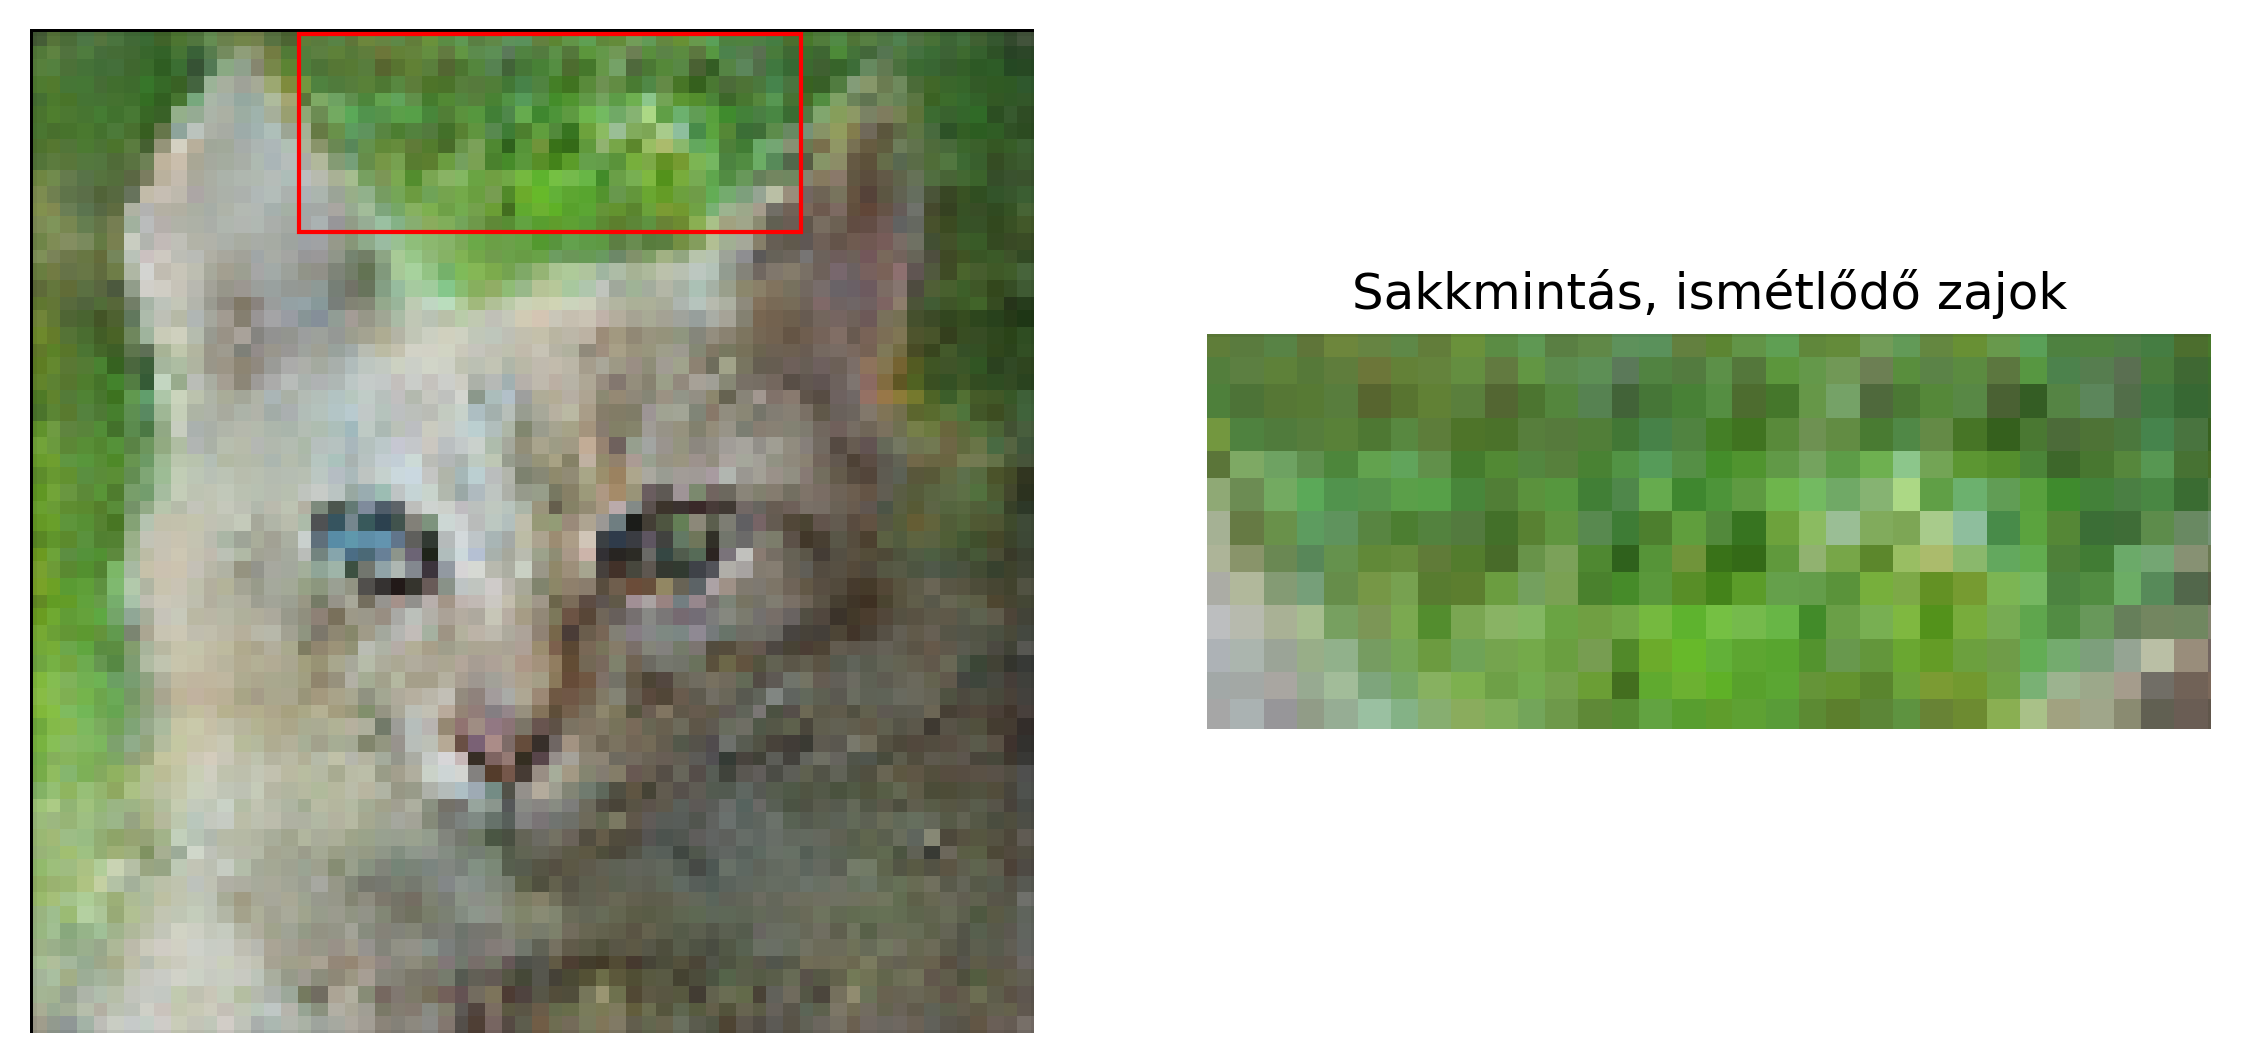
\includegraphics[width=13cm]{images/chessboard-patterns.png}
\caption{Jellegzetes zajok a generált képeken}
\label{fig:chessboard-patterns}
\end{figure}

https://distill.pub/2016/deconv-checkerboard/

A cikkben a Dekonvolúciós rétegek helyett a Konvolúciós és UpSampling rétegeket ajánlották bilineáris interpolációval. Vagyis a felbontásnövelési feladatot elvették a dekonvolúciós rétegtől és egy tanítható-paraméter nélküli rétegre bízták a feladatot, aminek csak annyi a szerepe, hogy a felbontást növelje. Ezzel az ötlettel a sakkmintás zajt igen jól leredukálták a generált képeken. A tanítás előtti Generátor kimenetén is megfigyelhető, hogy a kép "lágyabb", kevésbé rendezettebb, mint az előző példában.

Viszont így önmagában nem volt szerencsém a modellt tanulásra bírnom és a BatchNormalization regularizációs rétegeket kellett beékelnem a modellbe. A technikát és a további alkalmazott regularizációs eljárásokat egy másik fejezeben foglalom majd össze.

\begin{python}
def add_upsampling_unit(model,
                        filters, kernel_size):
    model.add(
        Conv2D(
            filters=filters,
            kernel_size=kernel_size,
            padding='same',
            activation="relu",
            kernel_initializer="he_normal"
        )
    )
    model.add(UpSampling2D())
\end{python}

\begin{figure}[h]
\centering
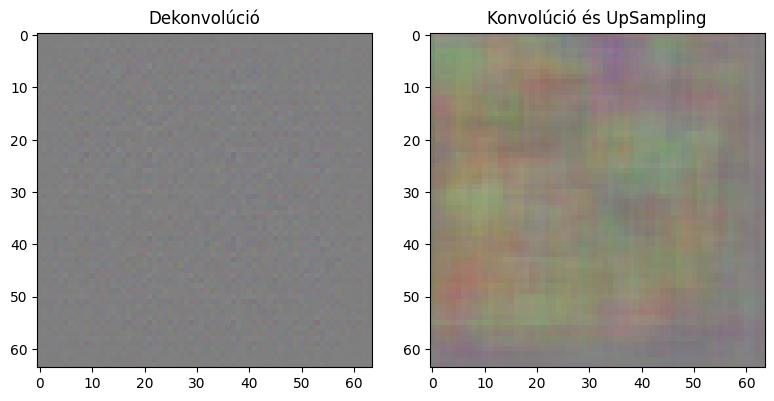
\includegraphics[width=13cm]{images/deconv-vs-conv_upsmpl.png}
\caption{Tanítás előtti Generátor kimenetei}
\label{fig:deconv-vs-conv_upsmpl}
\end{figure}
